% 73-83(73쪽) — 곡선 y=-x^2+9 와 x축의 두 교점 A, B · 선분 AB 를 한 변으로 하는 내접 사다리꼴(색칠). 스캔 화질이 낮아 TikZ 로 다시 그림.
% 원문에 있는 것만: 눈금 9(y축 꼭짓점) · 라벨 O, x, y, A, B, y=-x^2+9. 사다리꼴의 높이는 원문처럼 표시하지 않는다(답이 높이라서 눈금을 넣지 않는다).
% 사다리꼴 윗변 높이는 원문 그림의 비율(꼭짓점 높이의 약 0.7)을 그대로 따랐다 — 넓이가 최대인 자리가 아니다.
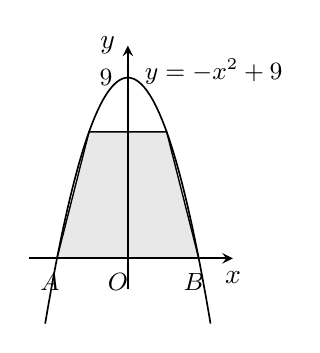
\begin{tikzpicture}[x=0.30cm, y=0.255cm, line width=0.5pt]
  % 색칠한 사다리꼴(아랫변 AB · 윗변은 곡선 위의 두 점)
  \fill[gray!18] (-3,0) -- (3,0) -- (1.643,6.3) -- (-1.643,6.3) -- cycle;
  \draw[line width=0.5pt] (-3,0) -- (-1.643,6.3) -- (1.643,6.3) -- (3,0);
  % 축
  \draw[->, >=stealth, line width=0.7pt] (-4.2,0) -- (4.45,0) node[below=1pt] {$x$};
  \draw[->, >=stealth, line width=0.7pt] (0,-1.5) -- (0,10.6) node[left=1pt] {$y$};
  % 곡선
  \draw[line width=0.6pt, domain=-3.5:3.5, samples=160, smooth] plot (\x, {9-(\x)*(\x)});
  % 라벨(원문 자리 그대로)
  \node[left=2pt, font=\small] at (0,9) {$9$};
  \node[anchor=west, font=\small] at (0.3,9.3) {$y=-x^2+9$};
  \node[below=2pt, font=\small] at (-3.3,0) {$\pt{A}$};
  \node[below=2pt, font=\small] at (-0.42,0) {$\pt{O}$};
  \node[below=2pt, font=\small] at (2.8,0) {$\pt{B}$};
\end{tikzpicture}
